\documentclass[12pt,a4paper]{article}\usepackage[]{graphicx}\usepackage[]{color}
%% maxwidth is the original width if it is less than linewidth
%% otherwise use linewidth (to make sure the graphics do not exceed the margin)
\makeatletter
\def\maxwidth{ %
  \ifdim\Gin@nat@width>\linewidth
    \linewidth
  \else
    \Gin@nat@width
  \fi
}
\makeatother

\definecolor{fgcolor}{rgb}{0.345, 0.345, 0.345}
\newcommand{\hlnum}[1]{\textcolor[rgb]{0.686,0.059,0.569}{#1}}%
\newcommand{\hlstr}[1]{\textcolor[rgb]{0.192,0.494,0.8}{#1}}%
\newcommand{\hlcom}[1]{\textcolor[rgb]{0.678,0.584,0.686}{\textit{#1}}}%
\newcommand{\hlopt}[1]{\textcolor[rgb]{0,0,0}{#1}}%
\newcommand{\hlstd}[1]{\textcolor[rgb]{0.345,0.345,0.345}{#1}}%
\newcommand{\hlkwa}[1]{\textcolor[rgb]{0.161,0.373,0.58}{\textbf{#1}}}%
\newcommand{\hlkwb}[1]{\textcolor[rgb]{0.69,0.353,0.396}{#1}}%
\newcommand{\hlkwc}[1]{\textcolor[rgb]{0.333,0.667,0.333}{#1}}%
\newcommand{\hlkwd}[1]{\textcolor[rgb]{0.737,0.353,0.396}{\textbf{#1}}}%

\usepackage{framed}
\makeatletter
\newenvironment{kframe}{%
 \def\at@end@of@kframe{}%
 \ifinner\ifhmode%
  \def\at@end@of@kframe{\end{minipage}}%
  \begin{minipage}{\columnwidth}%
 \fi\fi%
 \def\FrameCommand##1{\hskip\@totalleftmargin \hskip-\fboxsep
 \colorbox{shadecolor}{##1}\hskip-\fboxsep
     % There is no \\@totalrightmargin, so:
     \hskip-\linewidth \hskip-\@totalleftmargin \hskip\columnwidth}%
 \MakeFramed {\advance\hsize-\width
   \@totalleftmargin\z@ \linewidth\hsize
   \@setminipage}}%
 {\par\unskip\endMakeFramed%
 \at@end@of@kframe}
\makeatother

\definecolor{shadecolor}{rgb}{.97, .97, .97}
\definecolor{messagecolor}{rgb}{0, 0, 0}
\definecolor{warningcolor}{rgb}{1, 0, 1}
\definecolor{errorcolor}{rgb}{1, 0, 0}
\newenvironment{knitrout}{}{} % an empty environment to be redefined in TeX

\usepackage{alltt}
\usepackage{fullpage}
\usepackage{setspace}
    \doublespacing
%\usepackage[usenames,dvipsnames]{xcolor}
\usepackage{hyperref}
\hypersetup{
    colorlinks,
    citecolor=black,
    filecolor=black,
    linkcolor=blue,
    urlcolor=blue
}
\usepackage{dcolumn}
\usepackage{booktabs}
\usepackage{url}
\usepackage{tikz}
\usepackage{todonotes}
\usepackage[T2A]{fontenc}
\usepackage[utf8]{inputenc}
\usepackage[english]{babel}
\usepackage{graphicx}
\usepackage{caption}
\usepackage{subcaption}
\usepackage{afterpage}
\usepackage{xpatch}
\usepackage{csquotes}
\usepackage[style=authoryear, sorting=nyt, url=false, dashed=false, backend=bibtex]{biblatex}
\renewbibmacro{in:}{%
  \ifentrytype{article}{}{\printtext{\bibstring{in}\intitlepunct}}}
\renewbibmacro*{volume+number+eid}{
    \printfield{volume}
    \setunit*{\addnbspace}% NEW (optional); there's also \addnbthinspace
    \printfield{number}
    \setunit{\addcomma\space}
    \printfield{eid}}
\DeclareFieldFormat[article]{number}{\mkbibparens{#1}}


\renewcommand*{\bibpagespunct}{\addcolon\space}
\addbibresource{mybib.bib}
\IfFileExists{upquote.sty}{\usepackage{upquote}}{}
\begin{document}




\title{Why are More Trade-Open Countries More Likely to Repress the Media?}

\author{Justin Murphy\\
University of Southampton}

\maketitle

\begin{singlespace}
\begin{abstract}
Why are more trade-open countries more likely to repress the media, even though media freedom is positively correlated with most other components of globalization? To explore and understand this empirical puzzle, I argue that economic globalization exerts contradictory pressures on state-media relations. On the one hand, economic openness encourages national policymakers to promote media freedom because foreign investors are more likely to invest where information is reliable. On the other hand, because increasing globalization brings distributive conflict which can threaten governments, it also generates incentives for national policymakers to suppress information and communication. I argue that economic liberalization of trade, foreign direct investment, and foreign portfolio capital should increase the probability states will repress the media, as states seek to manage the domestic distributive conflicts generated by liberalization. However, while international \emph{investors} have a stake in the transparency of foreign countries, international \emph{traders} do not. Because of this, foreign investment should have a positive effect whereas trade openness should have a negative effect on media freedom, as investment corrects but trade enables the repressive tendency generated by liberalization. Furthermore, because portfolio capital is more mobile than foreign direct investment, the positive effect of portfolio capital should be greater than the positive effect of foreign direct investment. To test these expectations, I use a mixed-methods research design combining statistical analysis of a large panel of countries from 1972 to 2003 and within-case process-tracing on two hard cases: Argentina and Mexico in the 1990s.\footnote{Comments, questions, and feedback are welcome. Email: j.murphy@soton.ac.uk. Website: jmrphy.net. Twitter: @jmrphy.}
\end{abstract}
\end{singlespace}

\vspace{0.3cm}

Given the conventional wisdom that democratic political institutions drive economic openness \parencite{Milner:2005ci} and vice-versa \parencite{EICHENGREEN:2008gg}, it is surprising that since the 1970s, on average, those countries which have been more open to international trade have had lower levels of media freedom. Although overall economic globalization is positively correlated with media freedom around the world, the bivariate relationship between trade and media freedom is, surprisingly, weakly negative. Considering all countries between 1972 and 2003 for which there is available data, those which more often had a repressive media environment engaged in higher levels of international trade than those countries which more often had a free media. This is true in both democratic and non-democratic countries, although the negative relationship is weaker in democratic countries. Given the positive correlation found between media freedom and other measures of economic globalization such as foreign direct investment (FDI) and foreign portfolio investment (FPI), as well as the KOF index for overall economic globalization \parencite{Dreher:2008dg}, the coincidence of high trade openness and media repression is a surprisingly under-reported empirical puzzle in international and comparative political economy.

\afterpage{
\begin{figure}[t]
    \caption{Media Freedom and Trade vs. General Economic Globalization, 1972-2003}
    \label{absolute}
    \begin{center}
\begin{knitrout}
\definecolor{shadecolor}{rgb}{0.969, 0.969, 0.969}\color{fgcolor}

{\centering 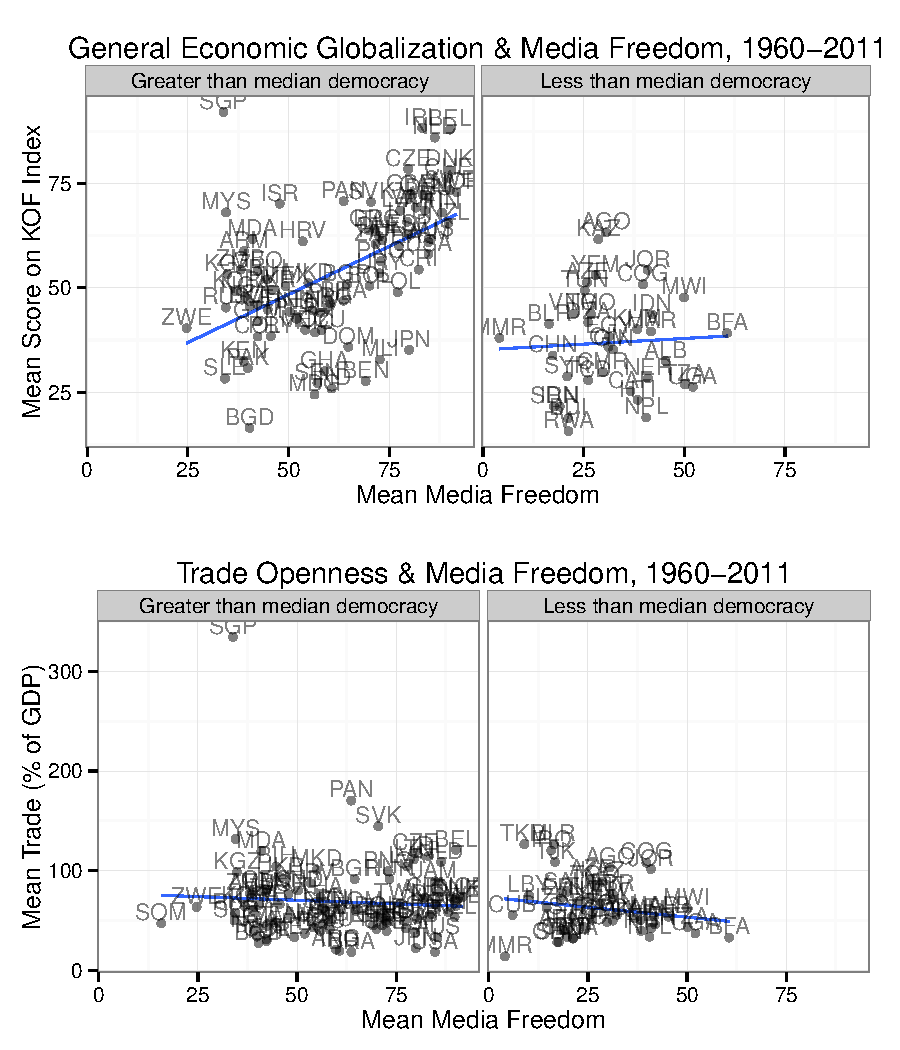
\includegraphics[width=\maxwidth]{figures/Intro} 

}



\end{knitrout}
    \end{center}
    \begin{singlespace}
        {\scriptsize{The KOF Index of Globalization is a 100-point scale reflecting the quantity of international trade and investment policy restrictions as well as flows of trade, FDI, FPI, and income paid to foreign nationals and capital \parencite[43]{Dreher:2008dg}. Media freedom is measured on a dichotomous scale (free or not free). See the section on Data and Method for a detailed description of the data sources. 
                      }}
    \end{singlespace}
\end{figure}
\clearpage
}

This puzzle points to a larger gap in research on the domestic effects of economic globalization. Scholars of international and comparative political economy (IPE/CPE) have not yet developed a serious theoretical and empirical account of how national media politics are likely to be affected by increasing integration of national economies. Much is known about the effects of economic integration on aspects of domestic politics such as cleavages \parencites{Rogowski:1987ip}{Rogowski:1989wm}{Hiscox:2002us}{hiscox2002international}, growth rates \parencite{Rodriguez:2001uw}; domestic spending \parencites{Rodrik:1998te}{Burgoon:2001dp}; civil war \parencites{Barbieri:2005uk}{Bussmann:2007vx}, and generic measures of democracy \parencites{EICHENGREEN:2008gg}{Li:2003vj}. But very little is known about how economic integration affects national media politics. One exception is an unpublished working paper by Orion Lewis \parencite*{Lewis:qDvYbWlU}, which finds mixed but suggestive evidence that trade openness is negatively related to media freedom and FPI is positively related to media freedom. Other research has considered whether political and civil liberties (broadly including freedom of the media) affect international economic flows \parencite{Adam:2007gn} and the effect of media in economic reform \parencites{Coyne:2004bq}{Islam:2002uc}. Yet scholars of international and comparative economy have not yet furnished any systematic analysis relating the different components and dynamics of globalization to the domestic politics of media freedom.

This article provides the first systematic investigation of how various components of globalization (specifically, trade, FDI, and FPI) shape the direction and dynamics of domestic media freedom. On the one hand, I argue that economic openness encourages national policymakers to promote media freedom because foreign investors are more likely to invest where information is reliable. On the other hand, because increasing globalization brings distributive conflict which can threaten governments, it also generates incentives for national policymakers to suppress information and communication. This paper outlines competing theoretical expectations from previous research and proposes a theoretical solution to reconcile these contradictory expectations. I argue that economic liberalization of trade and investment should increase the probability states will repress the media, as states seek to manage the domestic conflict it generates. However, while international \emph{investors} have a stake in the transparency of foreign countries, international \emph{traders} do not. Because of this, foreign investment should have a positive effect whereas trade openness should have a negative effect on media freedom, as investment corrects but trade enables the repressive tendency generated by liberalization. Furthermore, because portfolio capital is more mobile than foreign direct investment, the positive effect of portfolio capital should be greater than the positive effect of foreign direct investment.

To test these expectations, I use a mixed-methods research design combining statistical analysis of a large panel of countries from 1972 to 2003 and qualitative process-tracing on the cases of Argentina and Mexico. Binary time-sectional, cross-series (BTSCS) analyses and panel vector-autoregressions (PVAR) provide evidence that, unique among the components of globalization considered here, trade levels have a robustly negative association with media freedom in the long-run. The effects of foreign investment are also broadly consistent with expectations, though they are less straightforward. As predicted, FPI has a stronger positive effect on media freedom than FDI. However, the difference is even greater than predicted: surprisingly, FDI has a robustly negative long-run effect on press freedom in BTSCS and PVAR analyses. I find no evidence that economic liberalization of any kind increases the probability of media repression in the short-run. Finally, qualitative process-tracing on cases from Argentina and Mexico in the 1990s, selected as relatively hard cases of consolidating democracies which for that reason strongly predict media freedom, each provide some illustration of the mechanism relating trade openness to media repression.

The article makes three main contributions to research on the domestic effects of economic globalization and state-media relations. First, this article provides the first systematic investigation of an important but neglected set of relationships, placing a new set of questions regarding the globalization-media nexus into current political economy and media research agendas. Second, the findings contribute to research on the domestic politics of economic globalization and in particular research on the larger globalization-democracy nexus, highlighting when and how economic liberalization can call forth media repression as a significantly anti-democratic technique for negotiating domestic political conflicts. Third, the article will be of interest to scholars of state-media relations and public advocates of media freedom because very little media research to date has systematically accounted for the ways in which international economic pressures shape states' tendencies toward or away from media freedom.

The article proceeds in five sections. The first section reviews previous research at the intersection of globalization, democracy, and the media. The second section presents a simple informal model of a national policymaker facing domestic backlash for the distributive conflicts brought on by an increase in economic openness, and deducts four hypotheses differentiating the expected effects of trade, FDI, FPI. The third section explains the data, methods, and research strategy. The fourth section presents and discusses the quantitative and qualitative findings, and the fifth section concludes.

\section{Globalization, Democracy, and Media}

Previous research provides strong reasons to expect the global integration of markets to exert pressures on institutions of democracy, but there remains much theoretical uncertainty about the degree to which these effects are positive or negative. Many have argued that economic globalization generates economic growth which strengthens democratic institutions \parencites{Baghwati:1997vy}{Im:1996cl}, increases incentives for peace \parencites{Baghwati:1997vy}{Oneal:1999fc}, or diffuses democracy as a norm (Kant [1795] \cite*{Kant:1983uf}; \cite{Limongi:1996dr}). On the other hand, many have argued that economic globalization is negatively associated with democracy because it rewards efficiency rather than popular sovereignty \parencites{Huntington:1975vt}{Lindblom:1977ue}{Cammack:1998gf}, or because leaders may prefer to repress rather than compensate the domestic losers from increased openness \parencite{Adsera:2002vt}.\footnote{See \cite{Milner:2009hi} for a review of these debates.} Within the general debate surrounding the globalization-democracy nexus, some researchers such as Li and Reveuny \parencite*{Li:2003vj} have sought greater clarity by disaggregating the distinct types of international economic flows and considering them separately, but relying on standard aggregate measures of democracy. Li and Reveuny find that trade and portfolio capital have negative effects on democracy, while foreign direct investment and democratic norms have a positive effect, but their dependent variable of democracy is calculated with the common procedure of subtracting the Polity autocracy score from the Polity democracy score. Thus, despite much research on the relationship between economic globalization and democracy, and despite evidence that disaggregation is fruitful for understanding this nexus of relationships, relatively little is known about how different international economic flows affect the various institutions which separately constitute what we know as democracy.

In particular, very little research to date queries whether and how economic globalization shapes state policies regarding domestic media freedom. One exception is Lewis \parencite*{Lewis:qDvYbWlU}, who finds that FDI inflows are positively associated with press freedom, trade levels are negatively associated with media freedom, and portfolio capital inflows have no discernible effect on press freedom. But as a first investigation into this question and as a largely inductive effort to establish the statistical patterns, the theoretical interpretations of this article are mostly provisional. Additionally, Lewis considers only levels of trade and year-by-year inflows of FDI and portfolio capital, whereas recent research shows that the distinction between flows (year-to-year movements) and stocks (the sum of all previous flows) is crucial in researching the effects of foreign investment on repression \parencite{Sorens:2012hc}. As discussed above, Antonis and Fillapaois \parencite*{Adam:2007gn} consider the effect of civil liberties such as media freedom on FDI, but not whether FDI affects civil liberties.

However, previous research on the relationship between markets and media more generally provides a basis for theorizing the relationship between economic integration and media freedom. Broadly, one tradition argues that the spread of markets and freer media are positively associated \parencites{Habermas:1991vg}{Islam:2002uc}{Islam:2003tu}. However, an opposite tradition suggets that markets and the logic of profits and efficiency create incentives for authoritarianism \parencite{Huntington:1975vt}. With respect to media politics in particular, Gehlbach and Sonin \parencite*{Gehlbach:2011ky} show that larger advertising markets are associated with nationalization of private media because, they argue, the benefits of state control increase with the advertising market. If economic liberalization tends to enlarge advertising markets by spurring economic growth, then liberalization might increase the state's incentives to repress private media just as it increases incentives to nationalize it. Furthermore, international economic integration brings the threat of social and political backlashes \parencite{Bussmann:2007vx}, which may require the state to compensate the domestic losers from globalization \parencite{Rodrik:1998te} or, alternatively, repress them \parencite{Adsera:2002vt}.

On the other hand, the literature on 'competitive authoritarianism' suggests that increasing economic interdependence is one of the forces which has increasingly rendered traditional authoritarian repression unfeasible \parencite[60, 62]{Levitsky:2002gx}. As a country becomes increasingly integrated with the world economy, it increases the costs of overt authoritarianism by increasing the salience of international opinion, increasing the voice of domestic opposition, and increasing the number of domestic actors affected by international perceptions \parencite{Levitsky:2006ex}. For example, Fujimori in Peru in 1992 and Putin in Russia in 1993 failed in their efforts to overtly circumvent the legislature in part due to such international pressures \parencite[56]{Levitsky:2002gx}. International pressures against overt authoritarianism force regimes to adopt formally democratic institutions such as elections, but often leaves them free to violate human rights and civil liberties. For example, in the US-Mexico negotiations leading up to the North-American Free Trade Agreement, Mexican leaders made significant changes to present a front of democracy and respect for human rights to encourage investors, but there was no specific or formal conditionality which would have prohibited or even discouraged the repression of civil liberties if necessary.

At the same time, Levitsky and Way highlight the media as one of the four main arenas in which incumbent governments can contest and subvert international pressures to democratize. Competitive authoritarian governments may permit a formally independent and relatively free media, as in Peru, Serbia, Panama, or Nicaragua during the late 1980s and much of the 1990s, while engaging in alternative, more subtle tactics of repression, such as manipulative adminstrations of the law or tax code \parencite[53, 58]{Levitsky:2002gx}

While economic integration engenders distributive conflicts which tempt states to repress certain domestic groups at the same time it disincentivizes certain overt techniques of repression, governments around the world increasingly engage in strategic, authoritarian interventions into domestic media politics. Corrales and Westhoff \parencite*{Corrales:2006vz} find, for instance, that authoritarian regimes are more likely to develop television than internet, because television is more easily controlled. Additionally, many authoritarian regimes welcome the internet but actively pursue techniques of information control and manipulation on the internet in a networked fashion \parencites{MacKinnon:2011id}{Pearce:2012fm}. These findings show that however much economic integration is making certain forms of repression obsolete, newer and more subtle techniques of media repression remain both attractive and viable.

As Antonis and Fillapaois point out, and as Lewis also argues, research on the relationship between globalization and democratic institutions likely shows such contradictory results because different international economic flows exert different pressures. To build on this idea while advancing the literature beyond the limitations discussed above, the next section provides a more deductive account of precisely why we should expect various types of international economic openness to exert different effects on media freedom.

The present study improves on the limited previous research in two ways. First, the present study uses newly expanded economic and media freedom data, which together permit the most comprehensive quantitative analysis of these relationships to date. In particular, I use the newly released Global Media Freedom Dataset by Whitten-Woodring and Van Belle \parencites{Belle:1997wo}{van2000press} and newly expanded measures of economic openness from Sorens and Ruger \parencite{Sorens:2012hc} to analyze a large panel of countries from 1948 to 2009. Second, I distinguish between levels and changes (long-run and short-run effects) in a country's exposure to international economic flows, using traditional regression analysis as well as more sophistcated time-series methods for panel data.

\section{Theory and Hypotheses}

Based on the review of previous research regarding the domestic political effects of international economic flows and the media politics of competitive authoritarianism, I develop a simple, informal model of how state media policy should respond to trade, foreign direct investment, and portfolio capital flows. Consider a state which experiences a variable increase in some inward, international economic flow of trade, FDI, or portfolio capital. This increased flow will increase the income of certain domestic groups and decrease the income of others, according to well-developed open-economy expectations (discussed below). The increased economic flow can be thought of as random and exogenous or the result of conscious state policy such as lowering tariffs. If they are well-informed and mobilized, a domestic group which experiences a negative income shock from economic liberalization would demand that the policymaker either close the domestic economy or compensate the group for its income loss, or else face rebellion. The “rebellion” could be electoral if the state is a democracy or a violent insurgency if the state does not have institutions to facilitate peaceful change. After experiencing the international shock, the media, if free to do so, would report the protests of the aggrieved group and its causes, namely, increased national exposure to the international economy and its conflictual distributive consequences. However, if the media does not fully report the political context and consequences of the international shock, the group which suffered an income loss would not threaten rebellion at all. A free media, in other words, are essential for domestic losers from globalization to exercise power in the domestic politics around the distributive outcomes of economic globalization. Where there is a free media, domestic losers from globalization hold policymakers accountable, but where there the media are manipulated by government, the claims of aggrieved groups cannot exact concessions from holding policymakers accountable. This can be from either not reporting and therefore not informing domestic groups of the political-conflictual nature of globalization, or from silencing those claims if and when they are made.

After increased exposure occurs, the policymaker would prefer not to compensate the domestic group but prefers compensation to facing rebellion or closing the economy to \emph{ex ante} levels. The policymaker can close the political process to any competitors to obviate the political pressure to compensate them \parencite{Adsera:2002vt}, but the higher their level of integration, the more costly are overt types of repression \parencite{Levitsky:2002gx}. Supposing that a policymaker can choose among compensating the aggrieved domestic group, excluding competitors from the political process, or engaging in some repressive practices which vary on a continuum from overt to covert. In effect, we can conceptualize their utility function as including a penalty on overtness which increases with the country's economic integration, such that there is decreasing utility to overt forms of repression such as outright exclusion from the political process or government killings but this disutility approaches zero for repressive tactics which are relatively obscure such as the selective prosecution or financial targeting of opponents.

Among the less visible ways of exercising anti-democratic control, information-communication control will be uniquely attractive for the policymaker. This is because not only are repressive media tactics less severe than mass killings or canceling elections, but because control of the media could potentially tame international judgments independently by shaping what gets reported internationally. That is, control of the media can first minimize policymaker accountability for the adjustment costs of liberalization by suppressing domestic dissent, but policymakers could also reasonably expect that suppressing information at home would decrease the flow of negative information abroad, promoting their international image in part by repressively shaping their image at home. In summary, increasing linkages to other states and international pressures raise the cost of overt repression for liberalizing states, which increases the attractiveness of more subtle, lower-visibility tactics for suppressing dissent against liberalization. Repression of the media stands out as a uniquely attractive first because it is precisely such a relatively low-visibility, low-salience type of repression but also because if successful it would tend to lower negative visibility in general.

\subsection{Differences among foreign direct investment, portfolio capital, and trade}

The previous subsection argues that media repression is uniquely attractive to incumbents presiding over economic liberalization. However, the international actors who are the counterparties to a country's international exchanges are also strategic actors. When a government represses the flow of information and communication within its territory, these counterparties will respond strategically depending on how their particular investment in the country is affected by domestic freedom of information and communication. Given that these international counterparties have very different stakes in domestic media freedom depending on whether they are engaged in trade, foreign direct investment, or portfolio capital investment, the utility of media repression during economic liberalization will be conditioned according to a country's composition of exposure to these flows.

\subsection{Foreign Direct Investment}

FDI is defined as the private capital flows from one firm to an enterprise located in a country outside of the firm's home nation. FDI flows consist of equity capital, intercompany debt, and reinvested earnings, whenever the investment is sufficient to give the firm a controlling stake (typically 10\%) in the enterprise \parencites[9]{DirectInvestmentTechnicalExpertGroupDITEG:2004wa}[588]{Jensen:2003to}. Foreign direct investment is unique among other types of international investment in that FDI involves a longer-term committment and thus the interests of FDI investors are relatively more aligned with the long-term interests of host countries \parencites{Lipsey:1999tn}[588]{Jensen:2003to}. The standard economic theory of FDI suggests that firm-level investment decisions to invest directly in a foreign country are not based on relative factor endowments or comparative rates of return, but on domestic market imperfections which can be exploited by multinational corporations (MNCs) better than domestic firms \parencites{Hymer:1960vo}{dunning2013international}. The distributive consequences of FDI inflows are complex: FDI is typically thought to increase inequality between skilled and unskilled workers as MNCs tend to be technologically skill-biased relative to domestic firms \parencite{Feenstra:1997kx} and unskilled, subsistence farmers do not have the resources to become entrepreneurs \parencite{Basu:2007ir}. However, FDI is also thought to decrease overall domestic income inequality as an increase in the supply of capital relative to labor increases wages and reduces inequality between capital and skilled labor \parencite{Jensen:2007fr}. Jensen and Rosas present evidence that, because poor countries have relatively little skilled labor, FDI's effect on closing the gap between skilled labor and capital is likely to decrease inequality on net even if it increases inequality between skilled and unskilled labor. Thus, FDI inflows generate distributive conflict among skilled and unskilled labor, but are unlikely to generate highly salient distributive conflict overall. This expectation is borne out by research on the relationship between economic globalization and civil war. Bussmann and Schneider \parencite*{Bussmann:2007vx} find, contrary to their expectations, that inflows of FDI decrease rather than increase the likelihood of civil war onset.

Of the three types of international economic actors considered here, investors of FDI have a long-term stake in the conditions of a host country. Because of this, despite long-standing expectations that foreign direct investors prefer the efficiency of authoritarian regimes, the balance of evidence suggests that democracies draw greater FDI flows than autocracies because they are more credible \parencite{Jensen:2003to}. Some scholars have sought to extend this logic by arguing that FDI should be attracted to respect for human rights \parencite{Blanton:2007gu} have faced problems of measurement and missing data \parencite{Sorens:2012hc}. After accounting for these issues, Sorens and Ruger find no link between FDI and human rights. Thus, while formal democracy attracts FDI and FDI does not appear to generate intense distributive conflicts, neither does it appear to “punish” governments for violating human rights. Antonis and Filipaios find, consistent with Jensen, that FDI seeks strong political rights while its attraction to civil rights is hump-shaped such that FDI is associated with both high and low levels of civil rights \parencite*{Adam:2007gn}. One possible explanation of these inconsistencies is that the socially positive consequences of FDI (rewarding democracy and rule of law and decreasing civil war onset) occur at the same time as, or perhaps in part through, the repression of civil rights. This is consistent with the model outlined above, wherein the repression of a particular civil right (the freedom of expression) embodied in media freedom is repressed to dampen the domestic conflict which would otherwise lead to perhaps more severe types of repression.

Thus, there are competing expectations regarding whether increases in FDI should be associated with media repression or media freedom. FDI does not appear averse to violations of rights per se, and may be attracted to governments with low respect for civil rights, so it possible FDI exerts no effect or a negative effect on media freedom, especially as its relative immobility means that its threat of exit would be less credible than that of FPI. On the other hand, FDI might be positively associated with media freedom for the same reasons it is associated with democracy, namely that it tends towards states which are credibile and stable.

\subsection{Portfolio capital}

Portfolio capital is defined as the purchase of stocks and bonds of less than 10\% of the outstanding stock of foreign firms \parencites{kenen1994exchange}{Walther:1997wf}. The standard economic theory is that portfolio capital tends to flow where the rate of return on the target country's domestic assets is high relative to the riskiness of the investment \parencites[743]{mosley2003global}[685]{ISQU:ISQU420}. Portfolio capital is distinguished, compared to FDI, by its short-term, speculative nature. In a benchmark study of how portfolio investors evaluate political risks, Bernhard and Leblang \parencite*{Bernhard:2003kb} show that portfolio investors respond to changes in country's political system (such as elections), but not to the substance of those changes (for instance, partisanship). Brooks and Mosley \parencite*{Brooks:2007we} show that portfolio investors do respond to the substance of policymaking, such as partisanship and macroeconomic priorities, but only in low-information environments such as electoral turnovers. The effects of partisanship and macroeconomic policy on portfolio capital decrease when the political system itself is stable. The overall point is that portfolio investors are first and foremost interested in stability and predictability rather than particular policies, which only matter in periods when the predictability of the future is low.

Portfolio capital inflows tend to appreciate the domestic currency, which makes imports relatively cheaper in the home market and exports relatively more expensive to foreigners. This will harm exports, leading possibly to unemployment or decreases in wage levels in export-intensive industries. It will also make it harder for domestic firms to compete with relatively cheaper imports, also possibly leading to unemployment or wage decreases. Finally, cheaper capital imports can encourage skill-biased shifts in technology usage, increasing the incomes of skilled labor and decreasing the incomes of unskilled labor \parencites{Cragg:1996iy}{Ros:2000vy}. Finally, because portfolio capital is relatively liquid, the threat of sudden withdrawal by international investors is well-known to have highly negative macroeconomic effects, such as in Mexico in 1995 and Argentina in 2001.

Given the interests of governments and portfolio investors, governments may be inclined to repress the media in response to the distributive effects of portfolio capital for two reasons. First, inflows of portfolio capital will make governments more beholden to the prevention of systemic political risks such as general strikes, expropriations, or revolutions \parencite{Clark:1997jg}. This is consistent with anecdotal evidence of portfolio investors who prefer governments to repress social unrest. Neoliberal economic reforms including international liberalization are often followed by large increases in foreign portfolio capital, and there is anecdotal evidence that in some cases foreign investors demand repression explicitly, such as when Chase Bank's Emerging Markets Group circulated a memo urging Mexican President Ernesto Zedillo to “eliminate the Zapatistas” and their uprising in Chiapas in 1994 \parencite{Silverstein:1995wc}.

Second, given that policy is evaluated by foreign investors largely in light of what is already known about the government and its history, incumbents who preside over financial liberalization may be sufficiently trusted by foreign capital that relatively subtle tactics such as media repression would be unlikely to shake confidence, especially if it is in the interest of preventing larger disruptions such as rebellions. It may be objected that portfolio investors would dislike media repression because they rely on a reliable flow of information regarding the country's conditions, but through modern “news management” politicians can practice a highly nuanced kind of transparency for international observers and also effectively repress domestic media using underhanded tactics. Indeed, country's which are open enough to receive capital inflows are likely to already be relatively transparent in the ways most relevant to investors, and this transparency required to induce investment might even embolden the assertiveness of domestic media. This appeared to happen in Mexico during the 1980s and 90s \parencite{lawson2002building}. Portfolio investors can typically rely on international news sources which are less likely to be targeted within the host country (on account of their financial independence and being linked to another sovereign, such as that one in Argentina). Finally, portfolio investors often have access to private, elite channels which provide them with politically important information about foreign country conditions before it would even be reported by free media \parencite{Dube:2011ir}, perhaps making them insensitive to media freedom within the host country.

Thus, there are competing expectations regarding the effects of FPI opn media freedom, just as there are with respect FDI. As a country adjusts to the distributive effects of FPI, governments may be more likely to repress the media as a relatively discreet tactic of pacifying this conflict, consistent with investors' interests in stability. However, inflows of portfolio capital may in the long-run be associated with media freedom, as portfolio investors prefer high-information environments ceteris paribus. However, FPI is different from FDI in the crucial fact that it is more mobile and therefore represents a much more credible threat of exit in response to government behavior. Therefore, while the expectations regarding FDI and FPI are bi-directional, to the degree foreign investment has a disciplining effect on state-media relations favouring media freedom, this effect should be strongest for FPI.

\subsection{Trade}

Trade, defined simply as imports plus exports as the percentage of a country's gross domestic product, is unique among the previous two components of economic globalization in that the international counterparties have no direct economic stake in the social and political conditions of the home country. Put simply, trade is not an investment as are FDI and FPI. The standard economic intuition explaining trade flows, although many sophisticated variations and extensions have been developed, is still the well-known Ricardian theory of comparative advantage. Other things equal, countries will tend to specialize in producing for export those goods which they are most advantaged in producing, and import from foreign producers those goods which domestic producers are unable to produce as efficiently.

International trade theory and much research in political science provides well-established expectations regarding the distributive effects of a country increasing its exposure to international trade. The standard Stolper-Samuelson model (1941) expects that increasing trade openness increases the income of the domestically abundant factor while decreasing the income of the domestically scarce factor. Thus, in capital-rich countries (industrialized or post-industrial countries), increasing trade openness benefits capital and harms labor, whereas in capital-poor countries increasing trade openness is expected to benefit labor and harm capital owners. In his benchmark study on the political consequences of these distributive expectations, Rogowski \parencite*{Rogowski:1989wm} finds strong evidence that domestic political coalitions are empowered and disempowered by international trade as the Stolper-Samuelson model predicts. Hiscox \parencite*{Hiscox:2002us} further refines these expectations by showing that the history is more finely explained by distinguishing the relative mobility of factors: when domestic factors are relatively immobile within the domestic economy, we do not observe class-based cleavages but rather sector-based cleavages and cross-class alliances, as immobility weds the interests of labor and capital to their shared industry. In turn, the threat of distributive conflict from international trade has been found salient enough to explain domestic political outcomes as diverse as the size of welfare states \parencites{Cameron:1978vb}{Burgoon:2001dp} and the onset of civil wars \parencite{Bussmann:2007vx}.

The international counterparties to a country's international trade have a uniquely low stake in the political stability of the country, for the simple reason that the import and export of goods and services is not directly affected by the sanctity of civil rights such as freedom of expression or media freedom. Although emerging international norms of “corporate responsibility” and “fair trade” are increasingly visible in marketing for consumers in the wealthy democracies, these norms revolve around specific labor market issues such as child labor, “sweatshops”, and wages paid to workers in developing countries \parencite{Moore:2004gy}. Even if some consumers in the wealthy democracies are increasingly willing to pay for more humane production conditions in foreign countries (effectively an international tax on repressive production conditions), there is no evidence and little reason to believe that economic behavior in importing or exporting goods and services anywhere in the world is in any way responsive to the sanctity of significantly less salient civil rights such as media freedom. For instance, consumers in the global North may very well prefer to pay premiums for coffee explicitly labeled as “fair trade,” but this provides no reason to expect they would pay more or less depending on whether the exporting country's trade agreements were facilitated by media repression. Similarly, if exporters in one country benefit from lowered tarrifs in a foreign country, compared to FDI and portfolio investors, they have uniquely less at stake in the political consequences faced by the foreign country with rising imports.

Thus, trade openness should be associated with a higher probability of media repression as it generates domestic distributive conflict but exerts little conceivable pressure in favor of a free media. If true, this would explain the puzzlingly negative correlation between international trade and media freedom despite the positive association between media freedom and most other components of economic globalization.

\subsection{Summary of Hypotheses}

To summarize, the hypotheses of the preceding subsections can be stated concisely as follows.

H1: Trade openness decreases the probability of media freedom.

H2. FPI increases or decreases the probability of media freedom.

H3. FDI increases or decreases the probability of media freedom.


\section{Data, Method, and Research Strategy}

To assess the theory, this article pursues a mixed-method research design employing large-N statistical tests and qualitative within-case analysis on two historically important cases. The intuition behind this research strategy is that statistical analyses are necessary to disentangle the independent effects of each economic flow, especially in distinguishing between short-run and long-run effects, while qualitative analysis is necessary for establishing the existence of a causal process.

In the quantitative analyses, I use state-level economic data collected by Sorens and Ruger \parencite*{Sorens:2012hc} for the main independent variables of interest (FDI, FPI, and trade as percentages of GDP) for all available countries between 1976 and 2003. For the dependent variable, I use the Global Media Freedom Dataset by Whitten-Woodring and Van Belle \parencite{van2000press}{Belle:1997wo}, which is the most comprehensive measure of media freedom to date. The Global Media Freedom Database provides an ordinal measure of media freedom with four levels but this variable reduces to a dichotomous variable capturing the distinction between not free and ``functionally free'' media. Country-years which take a value of ``not free'' are those where it is unsafe to criticize the government in the media or the government directly controls all news media. Countries which take a value of ``functionally free'' are those where there may be ``social, legal, or economic costs'' to criticizing the government in the news media but criticism of government still regularly takes place.\footnote{For greater detail, see ``Guidelines for using the Global Media Freedom Dataset'' available from the authors.} The final data matrix used in the quantitative analyses is an unbalanced panel of 153 countries with time-series as long as 1971 to 2003.

To further investigate the quantitative findings and enhance our understanding of the key puzzle motivating this paper, a following section offers two within-case analyses which trace the process whereby trade liberalization is expected to exert pressure on domestic media freedom. For reasons of data availability and to help control for confounding spatial and temporal factors, I consider Argentina and Mexico in the period between 1993 and 2003, two "third-wave" democracies from the same region in the same time period. These countries are analytically well-suited for further examination because they both democratized beginning in the 1980s and were consolidating in the 1990s. In autocratic regimes, even if we observed instances where media repression follows economic liberalization, it would be hard to infer that liberalization caused media repression because the media repression could be a function of auotcracy in general. On the other hand, if media repression follows economic liberalization in countries which are otherwise politically liberalizing, it will be more credible to infer that economic liberalization was a causal factor. Indeed, Argentina and Mexico are least likely cases to expect media repression at this time because Argentina's Carlos Menem and Mexico's Carlos Salinas were championed by American politicians as models of democratic economic liberalization. If these celebrated cases of relatively democratic economic liberalization display evidence of the hypothesized mechanism, then it is likely to take place in less democratic liberalizations as well. Another reason why these are hard tests is that, on the scale of the Global Media Freedom Database, both of these countries during this time period had functionally free media. Leveraging Freedom House's continuous measure of media freedom and qualitative evidence, I ask whether it is possible to observe the mechanism at a finer granularity than that provided by the dependent variable in the quantitative analysis \parencite{FreedomHouse:2011vv}.\footnote{Freedom House measures press freedom on a continuous scale from 0 to 100 beginning in 1994.} This approach is therefore also a robustness check on the dichotomous dependent variable in the statistical models. Substantively, Latin America is an attractive region for further study because Latin America is typically considered the first region where democracies were able to implement politically difficult "stabilization" policies. In the 1970s, it was a puzzle how economic liberalization would ever be achieved in democratic settings, given the status quo bias of elected politicians and the popular support for protectionist policies. An implication of this paper's argument, however, is that even in formally democratic countries economic liberalization may in some cases induce anti-democratic tactics such as media repression. If this is argument is correct, then substantively it would be most rewarding to better understand these cases which the conventional wisdom holds to be relatively democratic success stories. Additionally, Mexico, unlike Argentina and many other Latin American countries, did not experience a deeply repressive military junta in the twentieth century. Thus, if it is plausible that a government's historical legacy of repression could alone make media repression in a later period more or less likely, then we can be confident this is not an unobserved variable generating outcomes in both Mexico and Argentina.

Specifically, I offer two short, “disciplined-configurative” case studies for the purpose of better understanding these historically important cases and to further test for the presence of a causal process \parencite[75]{george2005case}. I use a combination of structured, focused comparison and process-tracing, asking specific questions about the hypothesized process in each case and weighing the empirical results against what the theory expects. Specifically, I ask the following three questions. What was the policy background as well as the magnitude and timing of trade exposure? What was the magnitude and timing, if any, of social unrest and was it observably in response to the distributive effects of trade? What was the magnitude and timing, if any, of government efforts to restrict freedom of the media? After investigating the historical record, I outline the answers to these questions and discuss how well they fit the theoretical model.

\section{Quantitative Analysis}

Table 1 displays the results of 2 different logistic regressions assessing the probability of observing media freedom in country$_{it}$.\footnote{The tables in this article were generated in R using the \emph{stargazer} package \parencite{stargazerLaTeXcod:vw}.} Before analysis, all variables were rescaled by subtracting the mean and dividing by two standard deviations so that the displayed coefficients reflect the expected effect of a two standard-devation increase each independent variable, holding the others constant.\footnote{This makes the regression coefficients for continuous predictors directly comparably to binary predictors \parencite{Gelman:2008gz}.}. Each logistic regression is estimated using robust (heteroskedastic and autocorrelation consistent) standard errors.

\afterpage{

% Table created by stargazer v.5.0 by Marek Hlavac, Harvard University. E-mail: hlavac at fas.harvard.edu
% Date and time: Mon, Oct 06, 2014 - 16:49:17
\begin{table}[!htbp] \centering 
  \caption{Standardized Logistic Regressions: Media Freedom} 
  \label{} 
\footnotesize 
\begin{tabular}{@{\extracolsep{5pt}}lcc} 
\\[-1.8ex]\hline \\[-1.8ex] 
\\[-1.8ex] & (1) & (2)\\ 
\hline \\[-1.8ex] 
 Democracy level & 4.13$^{***}$ & 4.12$^{***}$ \\ 
  & (0.12) & (0.12) \\ 
  Democracy change & $-$0.13$^{*}$ & $-$0.15$^{**}$ \\ 
  & (0.07) & (0.07) \\ 
  GDP per capita & 0.63$^{***}$ & 0.34$^{**}$ \\ 
  & (0.11) & (0.15) \\ 
  GDP per capita change & 0.10 & 0.09 \\ 
  & (0.09) & (0.10) \\ 
  Spline 1 & 0.30 & 0.31 \\ 
  & (0.20) & (0.20) \\ 
  Spline 2 & 0.11 & 0.09 \\ 
  & (0.46) & (0.46) \\ 
  Spline 3 & 0.38$^{**}$ & 0.24 \\ 
  & (0.15) & (0.16) \\ 
  Trade level &  & $-$0.33$^{***}$ \\ 
  &  & (0.11) \\ 
  Trade change &  & $-$0.05 \\ 
  &  & (0.11) \\ 
  FDI level &  & $-$0.37$^{*}$ \\ 
  &  & (0.20) \\ 
  FDI change &  & 0.23$^{*}$ \\ 
  &  & (0.12) \\ 
  FPI level &  & 0.85$^{***}$ \\ 
  &  & (0.17) \\ 
  FPI change &  & 0.01 \\ 
  &  & (0.18) \\ 
  Constant & $-$0.90$^{***}$ & $-$0.84$^{***}$ \\ 
  & (0.19) & (0.19) \\ 
 N & 4,052 & 4,052 \\ 
Log Likelihood & $-$1,429.00 & $-$1,406.00 \\ 
AIC & 2,874.00 & 2,839.00 \\ 
\hline \\[-1.8ex] 
\multicolumn{3}{l}{$^{*}$p $<$ .1; $^{**}$p $<$ .05; $^{***}$p $<$ .01} \\ 
\end{tabular} 
\end{table} 

\clearpage
}
Model 1 represents a baseline model of media freedom as a function of only levels and first differences of democracy and GDP per capita, with a natural cubic spline of time to control for autocorrelation \parencite{Beck:1998wg}. Model 2 adds to the baseline model levels and changes of international trade, inward FDI, and inward FPI. Model 1 indicates that level of democracy and GDP per capita have positive effects on the probability of observing media freedom, but the estimated relationship between democratization and media freedom is negative. Level of democracy has a predictably positive association with media freedom and is statistically significant in all models. This suggests that while democratic states in the long-run are more likely to have free media, democratizing states tend to repress the media. The coefficients for the natural cubic splines are statistically insignificant except for the third.

Controlling for these baseline predictors of media freedom, Model 2 introduces indicators of economic globalization. Consistent with H1, the results reveal a negative coefficient for level of trade, statistically significant at a 99.9\% confidence level. However, the statistically insignificant coefficient for first differences of trade level suggests that liberalization of trade does not have immediate, short-run effects on the probability of observing media freedom. Considering FDI, Model 2 suggests that FDI increases the probability of media freedom in the short-run but decreases it in the long-run. Finally, Model 2 suggests FPI has a positive effect on media freedom in the long-run (the largest effect of all) but no effect in the short-run.
\afterpage{
\begin{figure}[t]
    \caption{Simulated Effect of Trade Level on Expected Probability of Media Freedom}
    \label{absolute}
    \begin{center}
\begin{knitrout}
\definecolor{shadecolor}{rgb}{0.969, 0.969, 0.969}\color{fgcolor}

{\centering 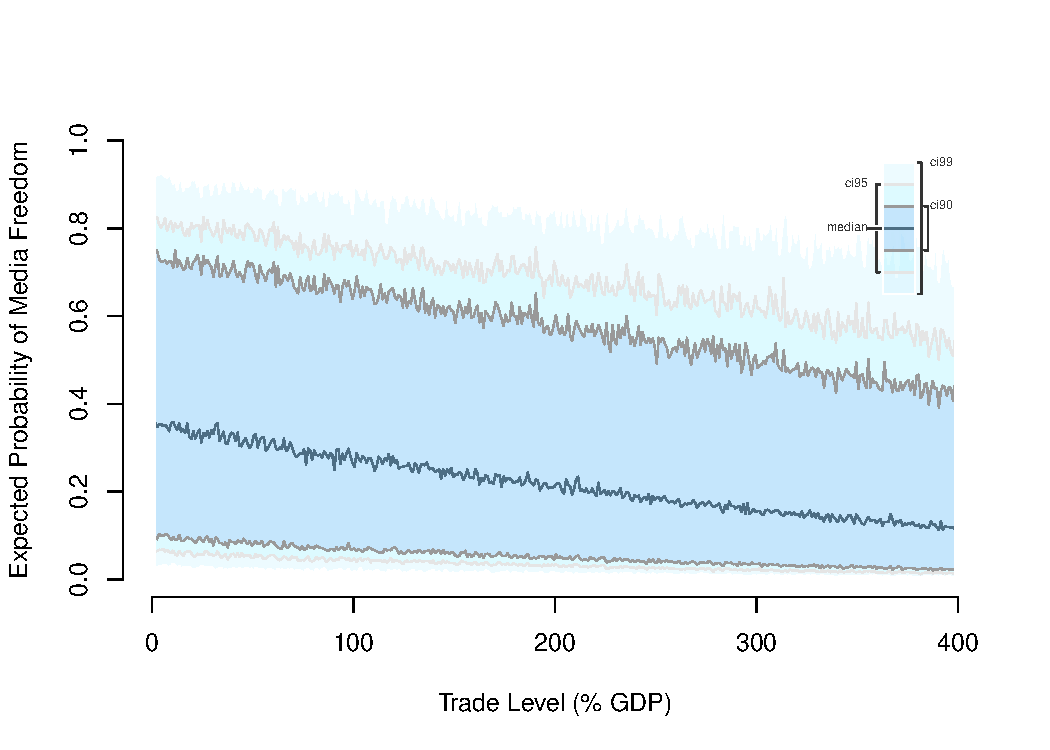
\includegraphics[width=\maxwidth]{figures/Trade_Effect_Plot} 

}



\end{knitrout}
  \end{center}
    \begin{singlespace}
        {\scriptsize{Expected values from 1000 simulations of Model 2 in Table 1.}}
    \end{singlespace}
\end{figure}
\clearpage
}

As logit estimates are not conveniently interpretable, Figure 2 illustrates how the expected probability of observing media freedom in $country_{it}$ changes as its level of international trade increases. The predicted probabilities are based on 1000 simulations of the model.\footnote{The simulations were conducted in R with the package \emph{Zelig} \parencite*{ZeligEveryonesSt:2009ts}}. The expected probability of observing media freedom in a country completely closed to international trade, with mean values on the other variables in the model, is .42. Increasing international trade from zero to 114.0024, which is one standard deviation above the mean of 68.4284, would be expected to decrease the probability of media freedom by \ensuremath{-0.0922} to .33.

\afterpage{
\begin{figure}[t]
    \caption{Simulated Effect of FDI Inflows on Expected Probability of Media Freedom}
    \label{absolute}
    \begin{center}
\begin{knitrout}
\definecolor{shadecolor}{rgb}{0.969, 0.969, 0.969}\color{fgcolor}

{\centering 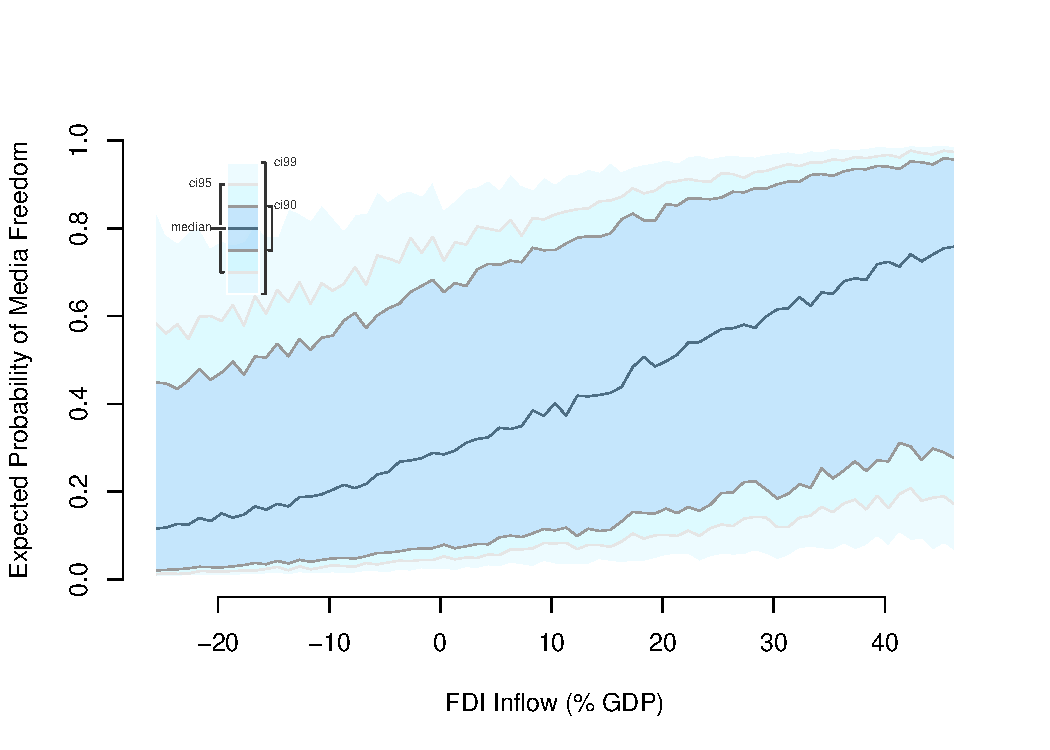
\includegraphics[width=\maxwidth]{figures/FDI_Effect_Plot} 

}



\end{knitrout}
  \end{center}
    \begin{singlespace}
        {\scriptsize{Expected values from 1000 simulations of Model 3 in Table 1.}}
    \end{singlespace}
\end{figure}
\clearpage
}


\afterpage{
\begin{figure}[t]
    \caption{Simulated Effect of FPI Stock on Expected Probability of Media Freedom}
    \label{absolute}
    \begin{center}
\begin{knitrout}
\definecolor{shadecolor}{rgb}{0.969, 0.969, 0.969}\color{fgcolor}

{\centering 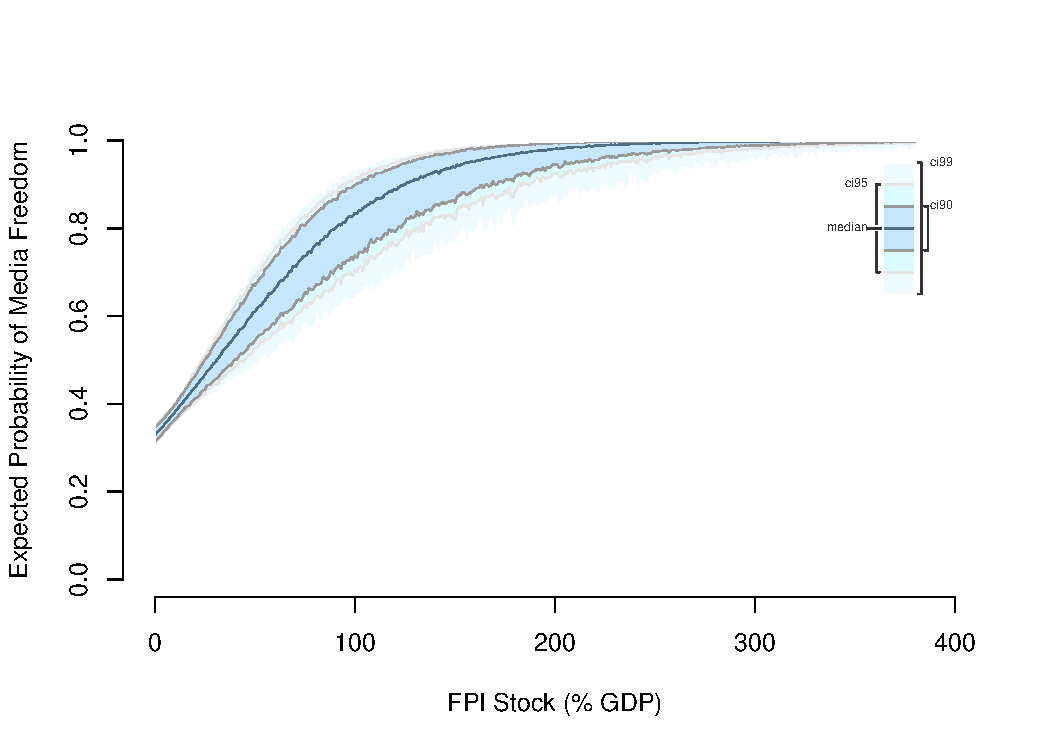
\includegraphics[width=\maxwidth]{figures/FPI_Effect_Plot} 

}



\end{knitrout}
  \end{center}
    \begin{singlespace}
        {\scriptsize{Expected values from 1000 simulations of Model 3 in Table 1.}}
    \end{singlespace}
\end{figure}
\clearpage
}



% 
% \afterpage{
% <<Interesting_Cases, results='asis', cache=FALSE>>=
% source("/Users/justin/Dropbox/gh_projects/globalization_media_freedom/analyses/explained_cases.R")
% require(stargazer)
% stargazer(model3.cases,
%           title="Cases Incorrectly Classified by Democracy and Domestic Economy but
%                       Correctly Classified by Adding Globalization Predictors",
%           style = "apsr",
%           summary=FALSE,
%           digit.separator=""
%                       )
% @
% \clearpage
% }
% 
% \afterpage{
% \begin{figure}[t]
%     \caption{Cases Unexplained by Democracy and Domestic Economy: Haiti, Malawi, Armenia, and Ukraine}
%     \label{absolute}
%     \begin{center}
% <<Explained_Cases_Plots, fig.align='center', cache=FALSE>>=
% source("/Users/justin/Dropbox/gh_projects/globalization_media_freedom/analyses/explained_cases_plots.R")
% grid.arrange(haiti_malawi_plots, ukraine_armenia_plots)
% @
% \end{center}
%     \begin{singlespace}
%         {\scriptsize{Grey shading indicates periods of media repression (\emph{Media Freedom} = 0).
%         International economic variables are measured as shares of GDP.
%         GDP per capita is divided by 100.
%         Freedom House Freedom of the Press Scores are on a 0-100 scale.}}
%     \end{singlespace}
% \end{figure}
% \clearpage
% }


\subsection{Robustness}

Vector autoregression (VAR) refers to an "*n*-equation, *n*-variable linear model in which each variable is in turn explained by its own lagged values, plus current and past values of the remaining *n* - 1 variables" (Stock and Watson 2001). VAR is ideal for checking whether the causal arrow of a hypothesis is properly directed, as it reveals straightforwardly whether changes in one variable typically precede changes in another variable or vice versa. Given its relatively atheoretical nature, VAR is an especially attractive tool for checking the robustness of a causal hypothesis against the historical record: while it would be dangerous to use VAR for inductively determining causal relationships, a true causal relationship would have to be consistent with the stylized facts of a VAR. A standard tool of econometrics since the 1980s, software implementations of VAR for panel data have only become available recently (Love 2006).

Panel VAR pools the time-series of multiple units (Hood et. al 2008; Hurlin and Venet 2001) as follows:

$$ y_{i,t} = \alpha_{i} + \sum_{k=1}^p \gamma^{(k)} y_{i,t-k} + \sum_{k=0}^p \beta_i^{(k)} x_{i,t-k} + v_{i,t} $$

for each of the cross-sections *i* and for all *t* in [1,T], where

$$ \gamma^{(k)} $$ represents the autoregressive coefficients and
$$ \beta_i^{(k)} $$ represents the regression coefficients

\afterpage{
\begin{figure}
\centering
\begin{subfigure}{.9\textwidth}
  \centering
  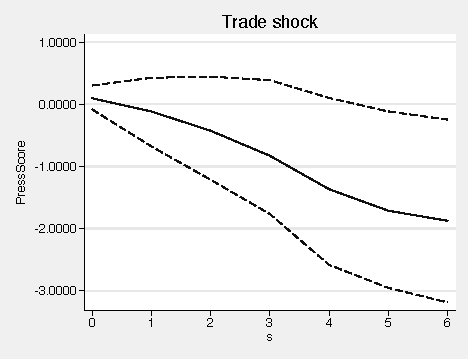
\includegraphics[width=.9\linewidth]{fhscore_response_to_trade.pdf}
  \label{fig:sub1}
\end{subfigure}
\begin{subfigure}{.9\textwidth}
  \centering
  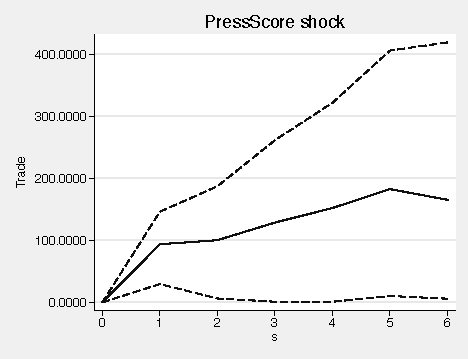
\includegraphics[width=.9\linewidth]{trade_response_to_fhscore.pdf}
  \label{fig:sub2}
\end{subfigure}
\caption{Impulse Responses From a Panel VAR}
\label{fig:testing}
\end{figure}
\clearpage
}

\afterpage{
\begin{figure}
\centering
\begin{subfigure}{.9\textwidth}
  \centering
  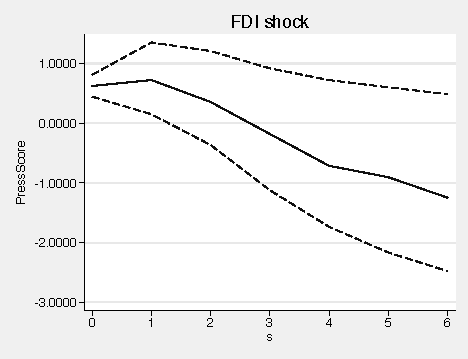
\includegraphics[width=.9\linewidth]{fhscore_response_to_fdi.pdf}
  \label{fig:sub3}
\end{subfigure}
\begin{subfigure}{.9\textwidth}
  \centering
  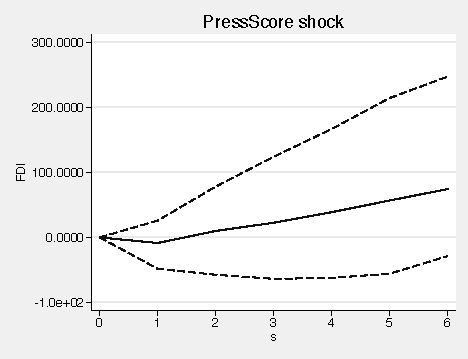
\includegraphics[width=.9\linewidth]{fdi_response_to_fhscore.pdf}
  \label{fig:sub4}
\end{subfigure}
\caption{Impulse Responses From a Panel VAR}
\label{fig:test2}
\end{figure}
\clearpage
}

\afterpage{
\begin{figure}
\centering
\begin{subfigure}{.9\textwidth}
  \centering
  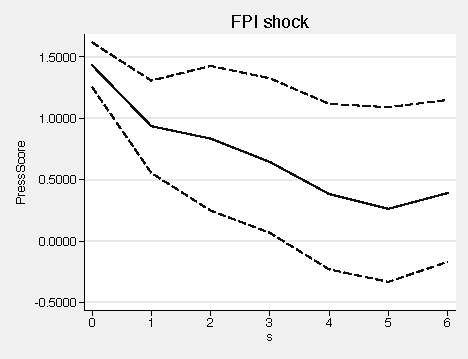
\includegraphics[width=.9\linewidth]{fhscore_response_to_fpi.pdf}
  \label{fig:sub5}
\end{subfigure}
\begin{subfigure}{.9\textwidth}
  \centering
  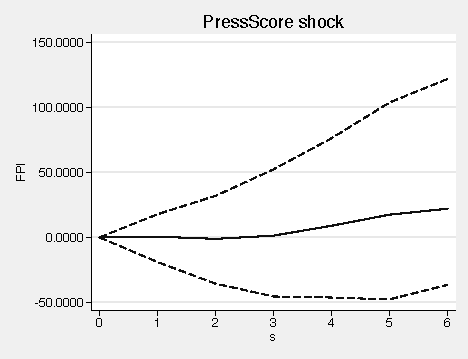
\includegraphics[width=.9\linewidth]{fpi_response_to_fhscore.pdf}
  \label{fig:sub6}
\end{subfigure}
\caption{Impulse Responses From a Panel VAR}
\label{fig:test3}
\end{figure}
\clearpage
}

\subsection{Qualitative Within-Case Analysis}

Next, I provide two brief case studies of Argentina and Mexico to assess qualitatively whether we can observe implications of trade liberalization generating pressures toward media repression.

\afterpage{
\begin{figure}[t]
    \caption{Globalization and Media Freedom in Argentina and Mexico, 1980-2003}
    \label{absolute}
    \begin{center}
\begin{knitrout}
\definecolor{shadecolor}{rgb}{0.969, 0.969, 0.969}\color{fgcolor}

{\centering 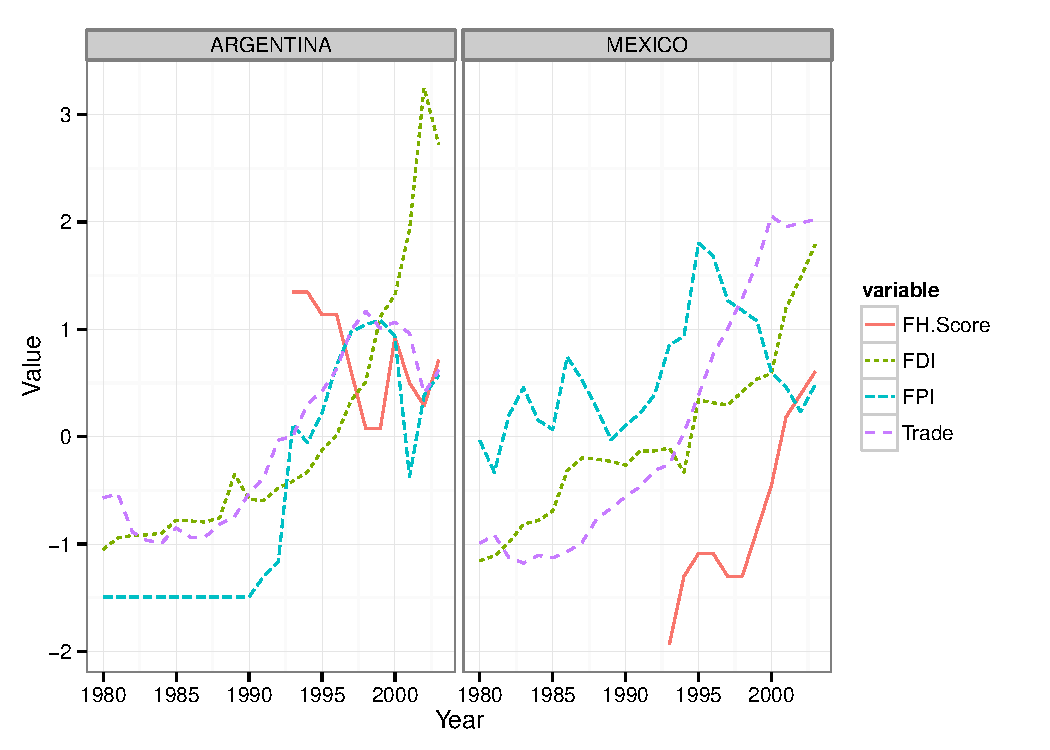
\includegraphics[width=\maxwidth]{figures/Case_Studies_Plots} 

}



\end{knitrout}
  \end{center}
    \begin{singlespace}
        {\scriptsize{Grey shading indicates periods of media repression (\emph{Media Freedom} = 0).
        Economic variables are measured as shares of GDP.
        Freedom House Freedom of the Press Scores are on a 0-100 scale.}}
    \end{singlespace}
\end{figure}
\clearpage
}

\subsubsection{Argentina}

Immediately upon inauguration as President in 1989, Carlos Menem announced a package of neoliberal economic reforms which include liberalization of international trade and capital flows, as well as privatizations and spending cuts. (Tommasi and Velasco 1995, 189; Borner and Kobler 2002). In the beginning of 1989, the average tariff rate is 39\% (a maximum import tariff was 50\% with a tariff surcharge of 15\% on all imports). By the end of 1989, the maximum tariff is 35\% and the average tariff rate falls to 12\%. In 1990, all import licensing requirements are abolished and tariffs are reduced across-the-board to 21\%. By 1995, the average unweighted tariff is 10.5\% and non-tariff barriers as well as export restrictions are removed (Beker 2011, 7).Exemptions were made for IT, domestic appliances, and autos. As a result, imports increased from \$4.1 billion in 1990 to \$21.6 billion in 1994, while exports increased from \$3.7 billion to \$20.1 billion at the same time. See Beker (2011).

As import competition put pressure on previously protected firms, about 30\% of manufacturing employment was destroyed between 1992 and 1996. In those industries where import penetration increased the most, wage inequality also widened during this period. Argentina's Gini coefficient for income inequality, one of the lowest in Latin America at the time, increased from 40.0 in 1991 to 47.4 by 1998. (Galiani and Sanguinetti 2003, 505; Beker 2011, 11)

Argentina will join the Mercosur customs union in 1991 and sign a trade agreement with the United States in 1994. The reform package largely succeeded in taming inflation rates and growing the economy. The inflation rate shrinks from 5\% in 1989 to .16\% by 1996 and gross domestic product grows by 40\% between 1990 and 1994 \parencite[4]{Beker:2011vq}. The IMF, World Bank, and the US government saw Argentina as a model student in this period \parencites[142]{Cavallo:2004bf}{Cavallo:2004ta}[167]{Klein:2002vg} and is frequently cited in leading global publications such as \emph{Time International} as a poster child for how neoliberal economic reforms should be implemented (\emph{Time International} \cite*{:3GmqDB3y}, as cited in \cites[194]{Echegaray:2001tf}{MarcusDelgado:2003gn}{Silverstein:2002wm}.

Although the reform package succeeds in taming Argentina's hyperinflation and creating economic growth, the most immediate and direct effect of trade liberalization was an increase in unemployment, especially among the workforce employed in previously protected, labor-intensive industries \parencite[10]{Beker:2011vq}. Additionally, trade liberalization reduced the income of small-scale producers who could not compete with cheap imports \parencite{eckstein2001power}. Although trade liberalization is costly to the sizable constituencies of unskilled industrial workers and rural campesinos, the government provides little public support for dislocated workers--reducing rather than increasing public spending--until the government develops a targeted income-assistance program during the currency crisis of 2001. This lack of government responsiveness between 1990 and 2001 is puzzling given the longstanding expectation that governments, and especially democratic regimes, must compensate domestic losers from liberalization in order to sustain a sufficient political coalition in favor of liberalization. This expectation should be especially strong for democratic governments, yet, despite the absence of government compensation, Argentina sees relatively little domestic conflict around trade liberalization. In fact, there are fewer strikes, strikers, and days lost to strikes than under Alfonsin \parencite{eckstein2001power}. Yet, dissent against liberalization was an observable current in public discourse in the years before Menem's repressive media regulations. It is worth noting that some of the media scandals related to government corruption were themselves linked to international economic openness. For instance, the aggressive Argentine daily Pagina/12, whose journalists were frequent targets of violence, sparked a scandal when they reported on the Menem administration requiring ``substantial payment" from the meatpacking firm Swift-Armour before they were allowed to import machinery into the country. Another highly publicized revelation involved the complicity of government officials in an international drug-laundering network \parencite{Waisbord:1994kq}. Most notably in road blockages organized by protesting farmers in 1991 and 1993, unfair international competition was a recurring point of dissent \parencites{McCullough:1991cs}{Ferber:1993fb}.

If the Menem regime neglected to make provisions for its harmed constituencies, how was it able to enact and sustain dramatic trade and capital liberalization in a formally democratic setting? The theory presented here expects that the Menem government is likely to repress the media in order to silence domestic opposition to liberalization while maintaining a formally democratic front. Consistent with the theory, the quantitative data reveal that after a long and stable period of stable economic openness and media freedom under Alfonsin, media freedom is volatile immediately after Menem's liberalization begins until it is stably repressed by 2005. According to a report Agresiones a La Prensa 1991-1994 published by the Asociacion Madres de Plaza de Mayo, around 452 acts of aggression were committed against the press between 1991 and 1994 (Delgado \cite*{Delgado:1995tr}, as cited in \cite[247]{Park:2002io}). Acts of aggression refer to “murder, death threats, bombings, bomb threats, intimidation, physical violence, violent threats, and termination of broadcasts.” If one were to count acts of excluding media from access to the government and public name-calling of the media by the government, the figure would be 546. Although not perpetrated directly by the state, during this period there were many acts of violence against investigative journalists critical of the Menem regime, acts which the government denounced but treated with impunity \parencite{Long:1993wb}. The Menem family's most direct actions against media freedom were cuts to state advertising in Pagina/12 \parencite[27]{Waisbord:1994kq}, 11 lawsuits against journalists under the pretense of criminal defamation \parencite{McCullough:1991cs}, proposals to increase libel and defamation sentencing, and a proposal to require media outlets to purchase prohibitively expensive libel insurance \parencite{Sims:kgMPqAHd}.

\subsubsection{Mexico}

As in the case of Argentina, Mexico's trade liberalization in the 1990s was part of a larger national project of neoliberal economic reform. Well before signing the North American Free Trade Agreement (NAFTA) with the United States and Canada in 1994, Mexico unilaterally lowered tarrifs from an average of 25\% in 1985 to 13\% by 1993 \parencites{McDaniel:2003kw}.

Concurrent with unilateral trade liberalization and NAFTA, and as in the case of Argentina under Menem, the Mexican government also privatized many state-owned enterprises and eliminated many state subsidies and price controls originally intended to support small farmers. Most subsidies for corn and wheat producers and retail food price controls were eliminatd by 1991 \parencite[295]{Hufbauer:2005vh}. In 1999, the Mexican government abolished CONASUPO, the state agency which bought staple crops at guaranteed prices and redistributed them to consumers \parencite[12]{Villareal:2010vk}.

After NAFTA, US imports from the US increased from \$50.8 in 1994 to 100.4 billion in 2000 \parencite[10]{Villareal:2010vk}. As in the case of Argentina, trade liberalization through the 1990s hurt small farmers and non-skilled manufacturing, as agricultural employment decreased from 8.1 million in 1993 to 6.8 million jobs in 2003, and value added decreased from \$32 billion to about \$25 billion in the same period.\parencites[289]{Hufbauer:2005vh}[14]{Villareal:2010vk}.

Also as in Argentina, increasing trade liberalization in Mexico led to increased wage inequality between skilled and non-skilled labor. In 1988, the real average wage level of skilled Mexican workers in the manufacturing sector was 225\% that of non-skilled workers. In 1996, it was about 290\% that of non-skilled workers, stabilizing until 2000 \parencite[9]{Villareal:2010vk}.

To support the transition into NAFTA, the government enacted the Programa de Apoyos Directos para el Campo (Program of Direct Support for the Countryside or “Procampo”), which provided farmers with direct, hectare-based income support. However, in part due to austerity following the peso crisis, total expenditure on Procampo decreased from \$1.4 billion to \$1 billion \parencite[295]{Hufbauer:2005vh}, despite the price of corn in Mexico falling from \$4.84 per bushel in 1993 to \$3.65 in 1997 \parencite[12]{Villareal:2010vk}, the total number of supported farmers decreased from 3.29 million to 2.95 million, between 1994 and 1998 \parencite[295]{Hufbauer:2005vh}.

On the day NAFTA went into effect in January 1994, the Ejército Zapatista de Liberación Nacional (EZLN) launched an armed uprising in one of Chiapas, one of Mexico's southernmost states. On that very first day of the uprising, EZLN spokesperson Subcomandante Marcos declared NAFTA to be “nothing more than a death sentence to the indigenous ethnicities of Mexico” and their uprising to be understood as a response “to the decree of death that the Free Trade Agreement gives them” (\emph{La Journada} 1994, as cited in \cite[216]{Hayden:2009uy}.

Although Procampo helped gain support for NAFTA, immediately there was popular discontent, such as in the Barzón Farmers movement in Zacatecas, regarding several inadequacies of the program, including payments not being made \parencite[173]{Williams:2001ux}. From 1993 to 1995, the Barzon movement sought and received much favorable attention in the print media, where reporters were not under great pressure to suppress reports \parencite[187]{Williams:2001ux}.

Neoliberal economic reforms, including increasing trade openness, somewhat surprisingly in light of our expectations although not exactly contradicting them, led to a relative opening of the domestic media \parencite{lawson2002building}. Between 1991 and 1993, in addition to pursuing NAFTA as his administration's top priority, Salinas' cuts to government spending included cutting the quid pro quo's which underwrote the traditional regime of media control. He specifically ended the system of paying for reporters accomodations on presidential trips, prohibited the distribution of bribes within the presidential palace, reduced the government advertising in which typically functioned as bribes for keeping media in line, ended tax deferments and credits to media, and stopped allowing media outlets to pay their Social Security taxes in advertisements. Privatization of state-owned enterprises also had the effect of reducing the media's dependence on government advertising revenues. The greater scrutiny from American and Canadian media relaxed the domestic media environment for domestic journalists, as it was easier for domestic journalists to report on topics that the foreign press were already reporting on outside any control from the Mexican government. Additionally, greater access to foreign inputs also freed the Mexican media from an important source of government leverage, in particular its traditional monopoly on the import of newsprint, providing further room for the Mexican media to take risks. As independent media outlets were gaining financial independence through market competition, at the same time the neoliberal state was relinquishing its traditional levers of control, led to a independence of the Mexican media increased significantly \parencite[76,89]{lawson2002building}.

The international spotlight from the NAFTA negotiations also forced Salinas to cultivate a more positive image on human rights, for instance, when he established the National Commission for Human Rights \parencite[107]{Dominguez:2009wd}. Additionally, because neoliberal economic reforms actually led to an opening of the media which the state could not control, Salinas and after him Ernesto Zedillo moved away from traditional tactics of media repression in favor of more modern techniques of “news management” and public relations, such as controlling information by only providing access to friendly reporters. For instance, in a 1990 press conference Salinas explicitly excluded several independent media outlets and only permitted the most reliable pro-government journalists. Later in 1996, the Interior Ministry for the first time created an explicit “blacklist” of journalists who government officials were supposed to not engage \parencite[39]{lawson2002building}.

Newspaper circulation is limited in Mexico, whereas television broadcasting dominated by Televisa is the main source of information, so it was dominated by pro-NAFTA, pro-government ideology \parencite{Hellman:1993wa}. They also used it for extensive foreign media campaigning. While building support for NAFTA, Salinas used media and PR tools extensively, including efforts to persuade Mexican-Americans and US investors to support NAFTA in the United States \parencite{Morris:2001iy}. This was the first time the Mexican government used advertising and lobbying in its foreign relations \parencite{Chabat:1997wj}. One of the most commented advertisements urged US business to look to Mexico as a place where they can hire workers for a dollar an hour \parencites[105]{center1993trading}[45]{Chabat:1997wj}.

This narrative reveals dynamics which are unexpected and in a crucial sense antithetical to our theory, for they reveal how economic liberalization may induce greater media freedom by increasing competition and growth. Yet, Salinas in particular was convinced that he had to protect the government's image to succeed in his foreign economic policies \parencite[107]{Dominguez:2009wd}. Although economic reforms made certain kinds of repression impracticable, under Salinas and then Zedillo the Mexican government engaged in specific acts to exclude the press from reporting on politically sensitive issues. Lawson observes plainly that Salinas was historically Mexico's “undisputed master of image management” \parencite[39]{lawson2002building}. Additionally, the editor of Mexico's Monitor, José Gutiérrez-Vivó, affirmed in 1996 that “Salinas was the president who was hardest on the media. He was the one who sought the most control over the media” \parencite[39]{lawson2002building}. After NAFTA passes, intimidation and direct violence against journalists at the hands of the state can still be observed, as when the state expropriates the property of critical editors \parencite{OrmeJr:1997da}. In fact, despite a de facto opening of the media due to financial independence and the neoliberal withdrawal of the state from private enterprise, federal state-media relations changed little until Zedillo and even his adminstration engaged in repressive tactics such as arresting the publisher of El Universal for tax-related reasons in 1996. Finally, physical assault against journalists increased throughout the period of Mexican media's opening from 1980 to the middle of the 1990s \parencite[81]{lawson2002building}, which was also a period of dramatic trade opening. Most of the physical assaults were not carried out by the government, but they were largely treated with impunity by the government.

Thus, in the process of trade liberalization, Mexican state officials actively seek greater control over the media as much as they can, despite the effect of increased competition unleashing an increasingly independent media. Both Salinas and Zedillo employed a variety of tactics ranging from traditional repression to modern “news management” in order to control their image in the media during a period of rapid trade liberalization. Salinas in particular, the earliest and most aggressive proponent of economic liberalization in the late 1980s and early 1990s, tried more than anyone else to control the media.

\section{Conclusion}

More trade-open countries are more likely to repress the media because increases in overall economic globalization generate incentives for national policymakers to repress the media and international trade is permissive of the continuation of this repression, whereas international capital investment is discouraging of continued media repression. This article provides a mix of quantitative and qualitative evidence suggesting that a country undergoing an increase in overall globalization is more likely to have a repressive media environment, even after controlling for previously well-established drivers of media freedom such as regime type, income, and economic growth. Several statistical models show further that, unique among the components of globalization considered here, trade levels have a robustly negative association with media freedom in the long-run. On the other hand, FDI and FPI appear to have a positive effect on media freedom, but their dynamics were somewhat puzzling: whereas FDI \emph{flows} exert a positive effect (in the short-run), \emph{stocks} of FPI have a positive effect on media freedom (in the long-run). Finally, qualitative process-tracing on cases from Argentina and Mexico in the early 1990s, selected as relatively hard cases of consolidating democracies which for that reason strongly predict media freedom, each provide some illustration of the mechanism relating globalization to the domestic politics of media freedom. The regimes of Carlos Menem in Argentina and Carlos Salinas in Mexico both saw media freedom decrease at moments illustrative of the theory.

Certain unexpected findings also suggest interesting questions. For instance, when economic liberalization increases market competition in the media sector (as it did in Mexico and Argentina), it generates strong pressures which favor a free, independent media. If this is the case, then it would provide a warrant for expecting trade liberalization to be associated with media freedom in the long run, as the conventional wisdom is that trade liberalization increases market competition. Thus, if trade indeed is associated with increased domestic competition, then it remains unclear why trade liberalization would be statistically associated with media repression in the long-run, a pattern evidenced in the statistical models here. One possibility is that the domestic economic and political consequences of trade liberalization are not fully understood and that trade liberalization independently is not associated with increased domestic competition.

The implications of this article are important for researchers of the globalization-democracy nexus because they highlight a specific way in which economic globalization can generate authoritarian tendencies.


\pagebreak

\section{Appendix}


% Table created by stargazer v.4.5.3 by Marek Hlavac, Harvard University. E-mail: hlavac at fas.harvard.edu
% Date and time: Sat, Apr 26, 2014 - 18:54:26
\begin{table}[!htbp] \centering 
  \caption{Variance Decomposition for Panel VAR} 
  \label{} 
\begin{tabular}{@{\extracolsep{5pt}} cccccc} 
\\[-1.8ex]\hline \\[-1.8ex] 
Variable & Democracy & Trade & FDI & FPI & PressScore \\ 
\hline \\[-1.8ex] 
Democracy & $0.952$ & $0.013$ & $0.014$ & $0.001$ & $0.020$ \\ 
Trade & $0.336$ & $0.612$ & $0.015$ & $0.008$ & $0.030$ \\ 
FDI & $0.196$ & $0.040$ & $0.743$ & $0.014$ & $0.008$ \\ 
FPI & $0.269$ & $0.059$ & $0.146$ & $0.523$ & $0.003$ \\ 
PressScore & $0.242$ & $0.025$ & $0.012$ & $0.009$ & $0.711$ \\ 
\hline \\[-1.8ex] 
\normalsize 
\end{tabular} 
\end{table} 


\begin{figure}[!htb]
\begin{center}
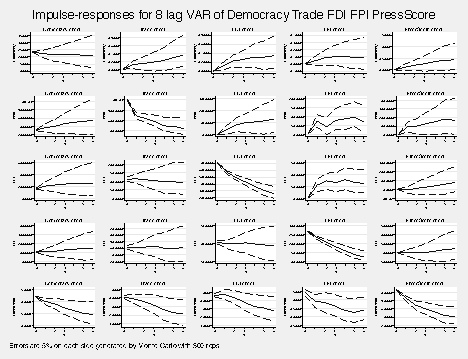
\includegraphics[width=1\textwidth]{grcombine1.pdf}
\caption{Digraph}
\end{center}
\end{figure}


\begingroup
\setstretch{0.8}
\setlength\bibitemsep{7pt}

\xpatchbibmacro{date+extrayear}{%
  \printtext[parens]%
}{%
  \setunit{\addperiod\space}%
  \printtext%
}{}{}



\printbibliography
\endgroup


\end{document}
